\chapter{La metafora}\index{metafora}
Nella linguistica cognitiva la metafora è definita come la comprensione di un dominio concettuale nei termini di un altro dominio concettuale, per esempio l'esperienza di vita di una persona nei confronti dell'esperienza di un'altra persona. Un dominio concettuale è una qualsiasi organizzazione coerente dell’esperienza.

Un esempio di metafora discusso da George Lakoff\index{Lakoff, George}\footnote{George Lakoff (24 maggio 1941) è un linguista statunitense, professore di linguistica (in particolare, linguistica cognitiva) all'Università di California Berkeley.} parte dalla frase ``la nostra relazione è in un vicolo cieco''. In questo caso l’amore viene concettualizzato come un viaggio. Non è un caso isolato: molte espressioni di uso corrente sono basate su questa concettualizzazione, e vengono usate non solo per parlare di amore, ma anche per ragionare a riguardo.

L'AMORE È UN VIAGGIO è una metafora mappata con la corrispondenza ontologica AMORE-COME-VIAGGIO, che mette in relazione la conoscenza sui viaggi con la conoscenza sull’amore. Dal punto di vista delle scienze cognitive bisogna chiedersi: esiste un principio generale che spiega come le espressioni linguistiche del viaggio sono usate per caratterizzare l’amore? Esiste un principio generale che governa come le inferenze sui viaggi possono essere usate nel dominio dell’amore?

La risposta ad entrambe le domande va ricercata nel fatto che la metafora può essere concepita come \emph{mapping}\index{mapping concettuale} (nel senso matematico del termine) da un dominio sorgente (in questo caso il viaggio) ad un dominio target (in questo caso, l’amore).

Va sottolineato che ciò che costituisce la metafora L’AMORE È UN VIAGGIO non è nessuna parola o frase in particolare, ma il mapping tra i domini concettuali. La metafora non riguarda quindi solo la lingua, ma anche i pensieri e il ragionamento.

\section{Mapping concettuale}
Una metafora concettuale si basa su due domini concettuali, dove un dominio viene compreso nei termini di un altro. Le espressioni metaforiche linguistiche sono parole o altre espressioni linguistiche che provengono dalla lingua o dalla terminologia del dominio concettuale concreto. Le metafore concettuali restano sottostanti alle espressioni metaforiche. 

Il dominio concettuale da cui sono tratte le espressioni metaforiche è detto \emph{dominio sorgente}. Il dominio concettuale che si tenta di capire è detto \emph{dominio obiettivo} o \emph{dominio target}.

Le metafore concettuali impiegano tipicamente un concetto astratto come obiettivo e un concetto concreto o fisico come sorgente. Ad esempio, metafore quali ``i giorni a venire'' oppure ``offrire il proprio tempo'' si affidano a concetti più concreti, esprimendo così il tempo (il concetto più astratto o target) come un (più concreto) percorso nello spazio fisico o come una sostanza che può essere presa o offerta in dono. Metafore concettuali differenti tendono ad essere invocate quando l'oratore tenta di sostenere un punto di vista o condotta di azione.

Il principio di unidirezionalità\index{principio di unidirezionalità} afferma che il processo metaforico va tipicamente dal concreto all'astratto, ma non nella direzione opposta. Di conseguenza, i concetti astratti sono compresi in termini di concetti-campione concreti.

Una mappatura è l'insieme sistematico di corrispondenze che esiste tra gli elementi costituenti dei domini sorgente e target. Molti elementi dei concetti target vengono dai domini sorgente e non sono preesistenti. Riconoscere una metafora concettuale significa riconoscere l'insieme di mappature applicabili ad un dato accoppiamento sorgente-target.

\section{Generalizzazioni}
La metafora L’AMORE È UN VIAGGIO è un mapping concettuale che caratterizza una generalizzazione di due tipi:
\begin{itemize}
  \item generalizzazione polisemica: generalizzazione sui significati delle parole;
  \item generalizzazione inferenziale: schemi di inferenza generalizzati su domini differenti.
\end{itemize}

\subsection{Espressioni idiomatiche}
Molte delle espressioni metaforiche discusse nella letteratura sono espressioni idiomatiche\footnote{Una espressione idiomatica è una espressione tipica di una lingua, solitamente intraducibile letteralmente in altre lingue se non col ricorso a espressioni idiomatiche della lingua in cui si traduce con significati affini alle espressioni idiomatiche della lingua da cui si traduce}. Nella linguistica cognitiva le espressioni idiomatiche non hanno un significato arbitrario. Ad esempio, ``girare a vuoto'' deriva da una convenzionale immagine mentale, quella di una ruota di un veicolo impantanato. Parte della conoscenza legata all’immaginario indica, ad esempio, che molta energia viene spesa nel far girare la ruota senza che alcun progresso avvenga. In sostanza, quando le espressioni idiomatiche hanno associata un’immagine convenzionale, è normale per la metafora mappare la conoscenza dalla sorgente al dominio target.

\subsection{Categorie superordinate}
Nel mapping L’AMORE È UN VIAGGIO la relazione amore corrisponde ad un veicolo. Il veicolo è una \emph{categoria superordinata} che include categorie base come automobile, treno, barca e aeroplano. Infatti, tutti gli esempi vengono presi da queste categorie di veicoli. Non è un caso: in generale il mapping avviene verso le superordinate invece che verso i livelli base.

Il mapping a livello superordinato massimizza le possibilità di mappare ricche strutture concettuali del dominio sorgente nel dominio target, dato che permette molte istanza a livello base, ognuna delle quali è ricca di informazioni.

\subsection{Categorie}
Le categorie classiche vengono capite metaforicamente come ``contenitori''. In questo senso ``qualcosa'' può essere dentro o fuori una categoria, può essere messo o rimosso da una categoria. La logica dei contenitori è che se X è nel contenitore A e A è nel contenitore B, allora X è nel contenitore B. Sotto la metafora LE CATEGORIE SONO CONTENITORI, le proprietà logiche delle categorie vengono ereditate dalle proprietà logiche dei contenitori. Uno dei metodi classici di ragionamento, il sillogismo, funziona ereditando le proprietà dei contenitori.

\subsection{Quantità e scale lineari}
Il concetto di quantità coinvolge almeno due metafore: DI PIÙ È SÙ e DI MENO È GIÙ (``i prezzi salgono'', ``le azioni crollano'', ecc).

Una scala lineare invece si può vedere in espressioni come ``la sua intelligenza va oltre quella del suo maestro''. La metafora LE SCALE LINEARI SONO PERCORSI mappa il punto iniziale di un percorso al fondo di una scala e la distanza percorsa alla quantità. La logica dei percorsi può essere quindi trasferita alla logica delle scale lineari. Ad esempio, se sto andando da Torino a Venezia lungo l’autostrada, e al momento sono a Milano, so che sono stato in tutti i posti da Torino a Milano (path inference). Se ho 50\euro, so di avere anche 20\euro, 30\euro{} e via dicendo e so di non avere 60\euro, 70\euro{} ecc.

Queste forme di inferenza sono le stesse, l’inferenza sul percorso è una conseguenza della topologia cognitiva dei percorsi.

\subsection{Il tempo come spazio}
È stato anche notato che si tende a concettualizzare il tempo come lo spazio. Il tempo viene quindi compreso in termini di oggetti (come entità e luoghi) e movimento (lo scorrere del tempo), partendo dal presupposto che il presente è il punto in cui si trova l’osservatore. Alcuni esempi possono essere siamo ``rimasti per tanto tempo'', ``è arrivato il momento'', ``ci avviciniamo al Natale''. Sempre in questo senso, il futuro si trova davanti all’osservatore e il passato dietro.

Possiamo distinguere due categorie a seconda che a muoversi sia il tempo (``si sta avvicinando il Natale'') o l’osservatore (``ci stiamo avvicinando al Natale'').

Molti aspetti della struttura degli eventi, incluse le nozioni di stato, cambiamento, processo, azione, causa, intento e significato, sono caratterizzate cognitivamente da metafore in termini di spazio, movimento e forza, secondo i seguenti mapping:
\begin{itemize}
  \item Stati sono luoghi
  \item Cambiamenti sono movimenti
  \item Cause sono forze
  \item Azioni sono movimenti spontanei
  \item Scopi sono destinazioni
  \item Mezzi sono cammini
  \item Difficoltà sono ostacoli
  \item Eventi esterni sono grossi oggetti che si muovono
\end{itemize}

\section{Principio di invarianza}\index{principio di invarianza}
Gli esempi visti fin qui ci portano a considerare il principio di invarianza: il mapping metaforico preserva la topologia cognitiva del dominio sorgente, in modo consistente con la struttura che eredita il dominio target. Quello che il principio di invarianza fa è garantire che, ad esempio, per la metafora dei contenitori, gli interni siano mappati con gli interni, gli esterni con gli esterni, i bordi con i bordi e via dicendo. Nella metafora dei path, le sorgenti vengono mappate con le sorgenti, gli obiettivi con gli obiettivi e via dicendo. Tutto questo va inteso come non tanto come ``copiare'' la struttura del dominio sorgente in quello target, quanto come pensare in termini di vincoli su corrispondenze fisse.

Infatti, i mapping metaforici mantengono le proprietà inferenziali soltanto se compatibili con il dominio target. Ad esempio, nella metafora LE AZIONI SONO TRASFERIMENTI, nella quale le azioni sono concettualizzate come oggetti trasferiti da un soggetto ad un altro, possiamo inferire che ciò che viene trasferito resta, mentre le azioni cessano di esistere dopo esser state compiute. Quindi, se diciamo che ``ti do un'informazione'', il principio di invarianza è rispettato e l'inferenza del significato avviene; se diciamo ``ti do un calcio'', il calcio non resta dopo averlo dato. In questo caso i vincoli del dominio target impediscono il mapping e la metafora non funziona.

\section{Dualità}
La \emph{dualità} viene individuata da Lakoff per la metaforizzazione di svariati concetti, in primis quello del tempo (TIME IS PASSING MOTION). In base a questa caratteristica un'unica metafora permetterebbe di dare luogo a concettualizzazioni speculari, corrispondenti rispettivamente al caso specifico ``TIME PASSING IS MOTION OF AN OBJECT'', dove il tempo che passa è il movimento di un oggetto rispetto a un osservatore fermo, e al caso specifico  ``TIME PASSING IS MOTION OVER A LANDSCAPE'', dove il tempo che passa è il movimento di un soggetto lungo un territorio. Questo fenomeno si rifletterebbe in mappature simultanee nell'arco di una stessa espressione, come ad esempio ``entro le settimane che arriveranno''. Questa è una frase in cui due parti distinte fanno uso di due distinti mapping in una volta sola. “Entro” fa uso della metafora secondo cui il tempo è un panorama statico con confini definiti, mentre “che arriveranno” fa usa della metafora del tempo come movimento. Ci si riferisce a queste coppie di mapping con il termine duali o mapping simultanei. Nella poetica si fa un largo uso di queste strutture.

\section{Realizzazione delle metafore}
L’uso delle metafore è talmente vasto che esso si estende anche oltre il linguaggio. I termometri, ad esempio, sono costruiti seguendo la metafora MORE IS UP. Altri esempi notevoli sono:
\begin{description}
  \item[Fumetti]bollire dalla rabbia (figura \ref{fig:metafora-rabbia})
  \item[Società]tempo è denaro (sta sprecando il suo tempo)
  \item[Legge]persone giuridiche
  \item[Politica estera]stati come persone
  \item[Forme discorsive]litigio come guerra
  \item[Pratiche sociali]vedere come toccare (gli occhi incollati alla tv)  
  \item[Rituali]sollevare i bambini appena nati  
  \item[Letteratura]viaggi come crescita  
  \item[Sintomi fisici]difficoltà sono pesi  
  \item[Interpretazione dei sogni]  
\end{description}

\begin{figure}[hbt]
  \centering
  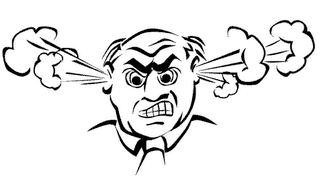
\includegraphics[width=0.6\textwidth]{img/metafora-rabbia.png}
  \caption{Esempio di metafora visuale RABBIA È PRESSIONE nella quale la rabbia viene rappresentata come ``vapore di una pentola a pressione''}
  \label{fig:metafora-rabbia}
\end{figure}

Possiamo concludere che in generale le metafore hanno dei costi (ad esempio, richiedono dei tempi più lunghi di lettura), ma anche grossi benefici in termini di comprensione e durata dei ricordi.
